\documentclass[11pt]{beamer}
% \usetheme{Copenhagen}
\usetheme{PaloAlto}
\usepackage[utf8]{inputenc}
\usepackage[spanish]{babel}
\usepackage{amsmath}
\usepackage{amsfonts}
\usepackage{amssymb}
\usepackage{graphicx}
\graphicspath{{figures/}}
\usepackage{ragged2e}
\usepackage{xcolor}
\usepackage{hyperref}
\hypersetup{urlcolor=blue}
\author{Carlos Espinosa}
\title{Partes de una computadora}
%\setbeamercovered{transparent} 
%\setbeamertemplate{navigation symbols}{} 
\logo{
\includegraphics[width=1.4cm]{fac-logo-w}} 
\institute{Facultad de Ciencias \\ Universidad Nacional Autónoma de México} 
\date{Agosto, 2022} 
% \subject{} 

\justifying
\begin{document}

\begin{frame}
\titlepage
\end{frame}

\begin{frame}
	\tableofcontents
\end{frame}

\section{Introducción}
	\subsection{Partes de una computadora}
		\begin{frame}{Partes de una computadora}
			Una computadora tiene dos componentes principales: \textit{hardware} y \textit{software}
			\begin{block}{Hardware}
				Todas las partes físicas y tangibles de una computadora, sus componentes eléctricos, electromecánicos y mecánicos; sus cables, gabinetes o cajas, periféricos de todo tipo y cualquier otro elemento físico involucrado.
			\end{block}
			\begin{block}{Software}
				Es todo el equipamiento lógico o soporte lógico de una Computadora digital, y comprende el conjunto de los componentes necesarios para hacer posible la realización de tareas específicas
			\end{block}
		\end{frame}
	\subsection{Hardware de una computadora}
		\begin{frame}{Hardware}
			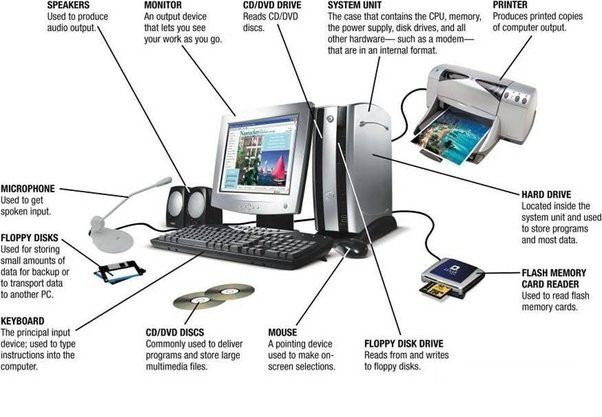
\includegraphics[width=\textwidth]{hardware.jpg}
		\end{frame}
		\begin{frame}{Categorías del \textit{hardware}}
			\begin{itemize}
				\item Unidad de procesamiento central (CPU)
				\item Almacenamiento
				\begin{itemize}
					\item Primario: Cache,Ram
					\item Secundario: Disco duro, desmontables (USBs)
				\end{itemize}
				\item Entrada/Salida (I/O)
				\begin{itemize}
					\item Dispositivos de entrada
					\item Dispositivos de salida
				\end{itemize}
			\end{itemize}
		\end{frame}
\section{Categorías del hardware}
	\subsection{Unidad de procesamiento central}
		\begin{frame}{Unidad de procesamiento central}
			La unidad de procesamiento central, también llamado procesador es el \textit{cerebro} de la computadora.
			
			\begin{center}
				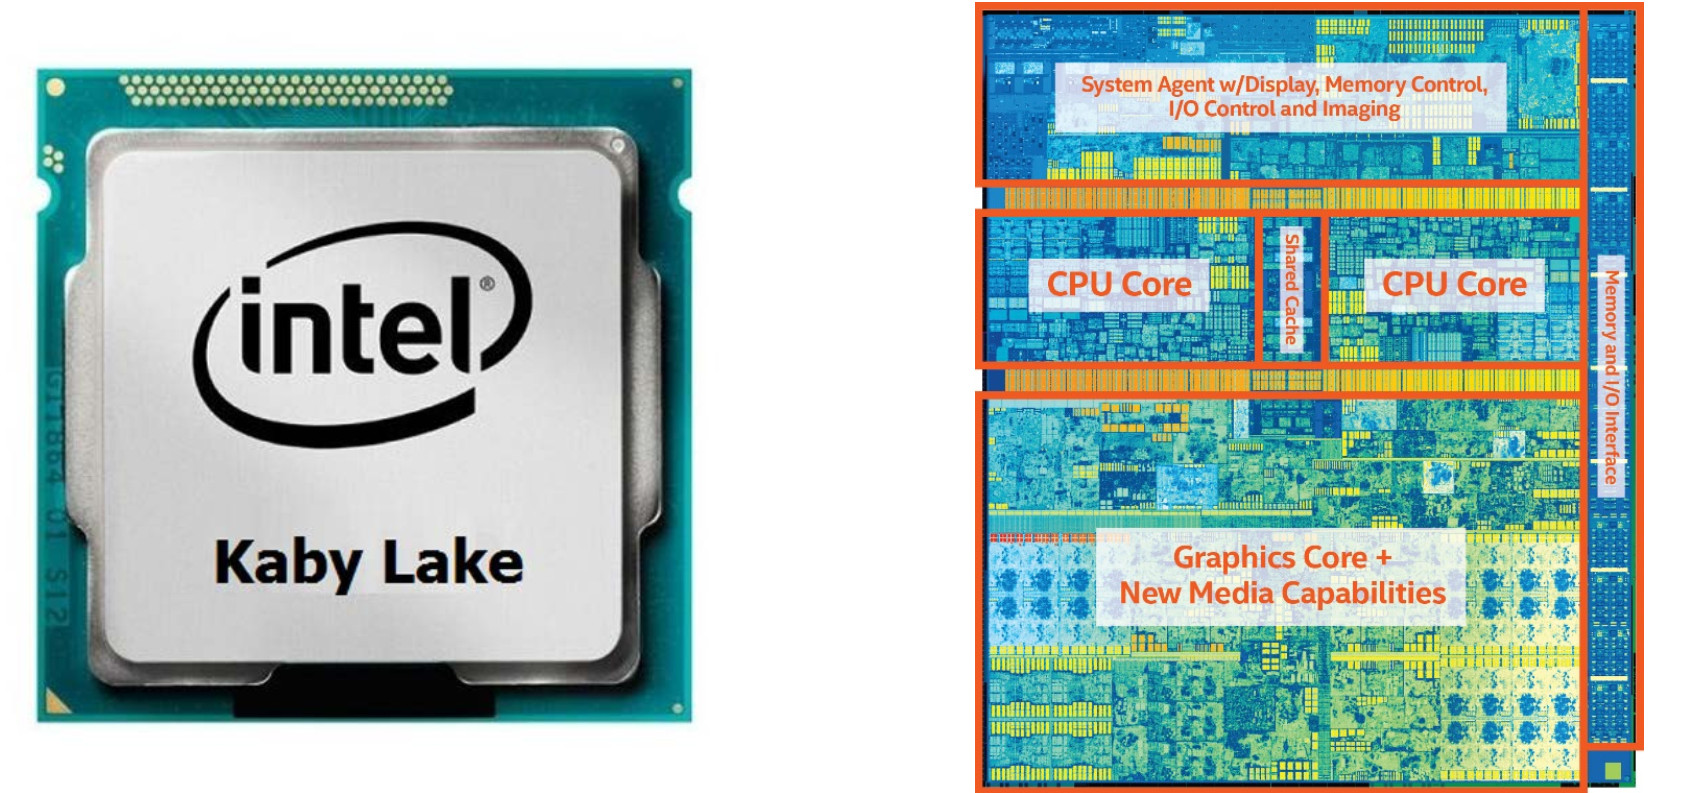
\includegraphics[scale=0.67]{cpu.jpg}
			\end{center}
			
			Se le llama arquitectura a el diseño del procesador. Esto determinará que software puede correr la computadora o que componente de hardware son admitidos.
		\end{frame}
		\begin{frame}{Ejemplos de arquitectura de CPU}
			\begin{itemize}
				\item x86: Intel Celeron/Pentium,/core/Atom/i3/i5,i7/Xeon y AMD Athlon/Sempron/Turion/<Phenom/Opteron/EPYC.
				\item ARM (en el 95\% de los teléfonos inteligentes y en algunas tabletas)
				\item IBM POWER9 (en servidores)
			\end{itemize}
			Existen otros procesadores que son utilizados para servidores principalmente.
		\end{frame}
		\begin{frame}{Partes de un procesador}
			El procesador consiste de tres partes principales:
			\begin{itemize}
				\item Unidad de Control
				\item Unidad lógica/aritmética
				\item Registros
			\end{itemize}

			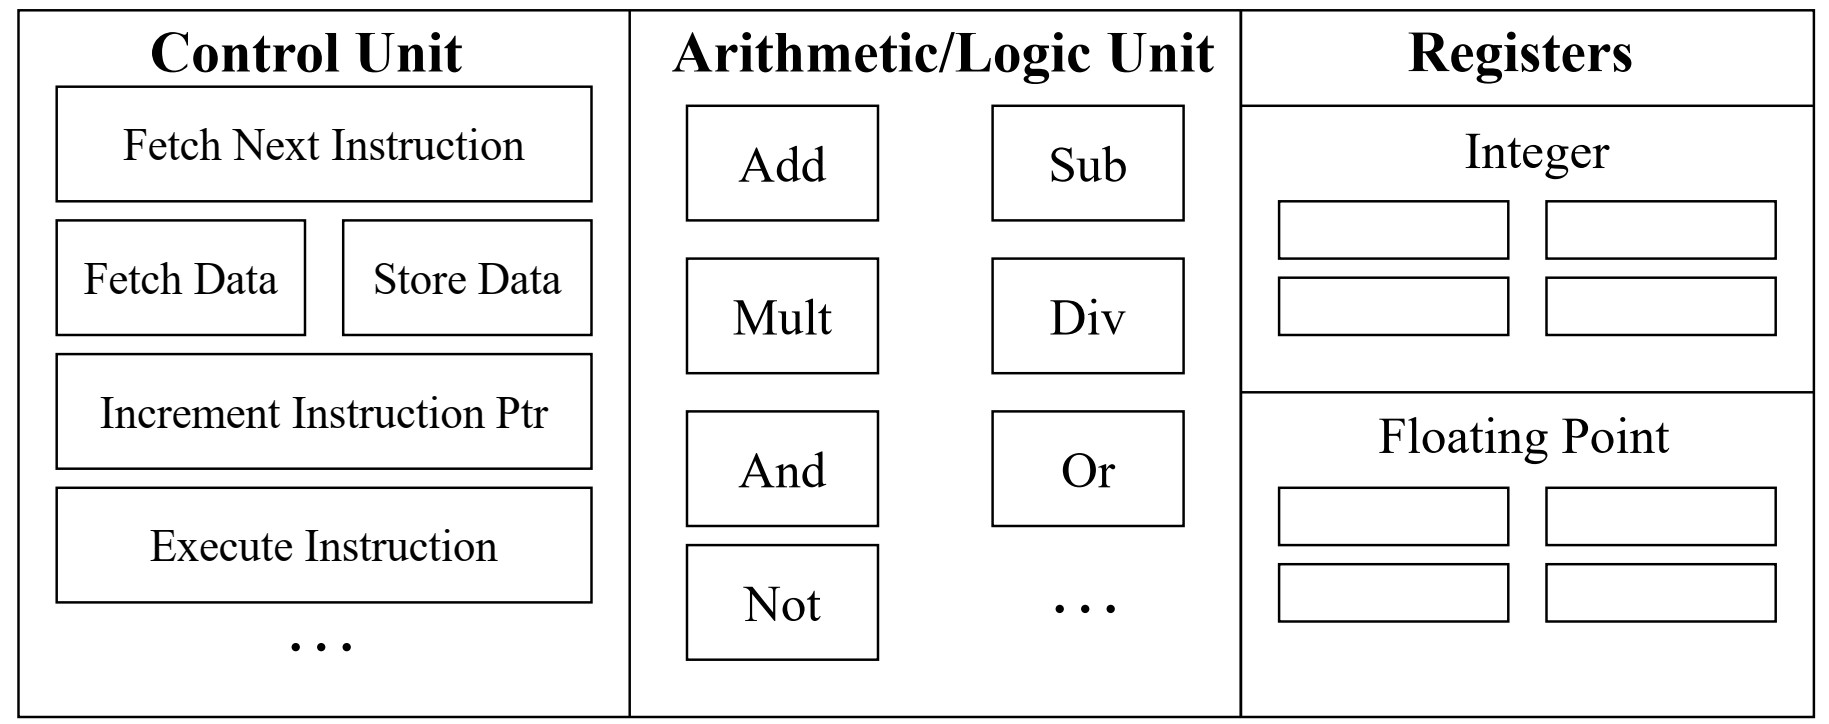
\includegraphics[width=\textwidth]{cpu_parts.jpg}

		\end{frame}
		\begin{frame}{CPU: Unidad de control}
			La unidad de control decide que hacer a continuación.
			
			Por ejemplo:
			\begin{itemize}
				\item Operaciones de memoria
				\begin{itemize}
					\item Carga de información de la memoria principal (RAM) a los registros.
					\item Guarda información de los registros a la memoria principal.
				\end{itemize}
				\item Operaciones aritméticas/lógicas
				\item Escoge entre varios caminos posibles de acción.
			\end{itemize}
		\end{frame}
		\begin{frame}{CPU: Unidad aritmética/lógica}
			La unidad aritmética/lógica realiza operaciones aritméticas y lógicas.
			\begin{itemize}
				\item Operaciones aritméticas: suma, resta, multiplicación, división, raíz cuadrada, coseno, etc.
				\item Operaciones lógicas: comparar dos números y ver cual es el más grande, revisar si un comando es verdadero, etc.
			\end{itemize}
		\end{frame}
		\begin{frame}{CPU: Registros}
			Los registros es la \emph{memoria} dentro del CPU donde está la información y las instrucciones que serán usadas de inmediato.
			
			Los registros contienen los operandos que se usarán en las operaciones (aritméticas o lógicas) que se están realizando en ese momento o también contendrá el resultado de alguna operación que acaba de ser realizada.
			
			Por ejemplo, si el CPU suma dos números, entonces:
			\begin{itemize}
				\item Uno de los sumandos será guardado en un registro.
				\item Otro de los sumandos estará guardado en otro registro.
				\item Después de realizar la suma, el resultado será guardado en otro registro.
			\end{itemize}
			Un CPU típico tienen solamente algunos cientos de bytes en los registros.
		\end{frame}
		\begin{frame}{Como son usados los registros?}
			\begin{itemize}
				\item Cada operación aritmética o lógica tiene uno o mas operandos y un resultado
				\item Los operandos están guardados en registros (La fuente)
				\item Una \textit{caja negra} de circuitos realiza la operación.
				\item El resultado se guarda en un registro (Destino)
			\end{itemize}
			
			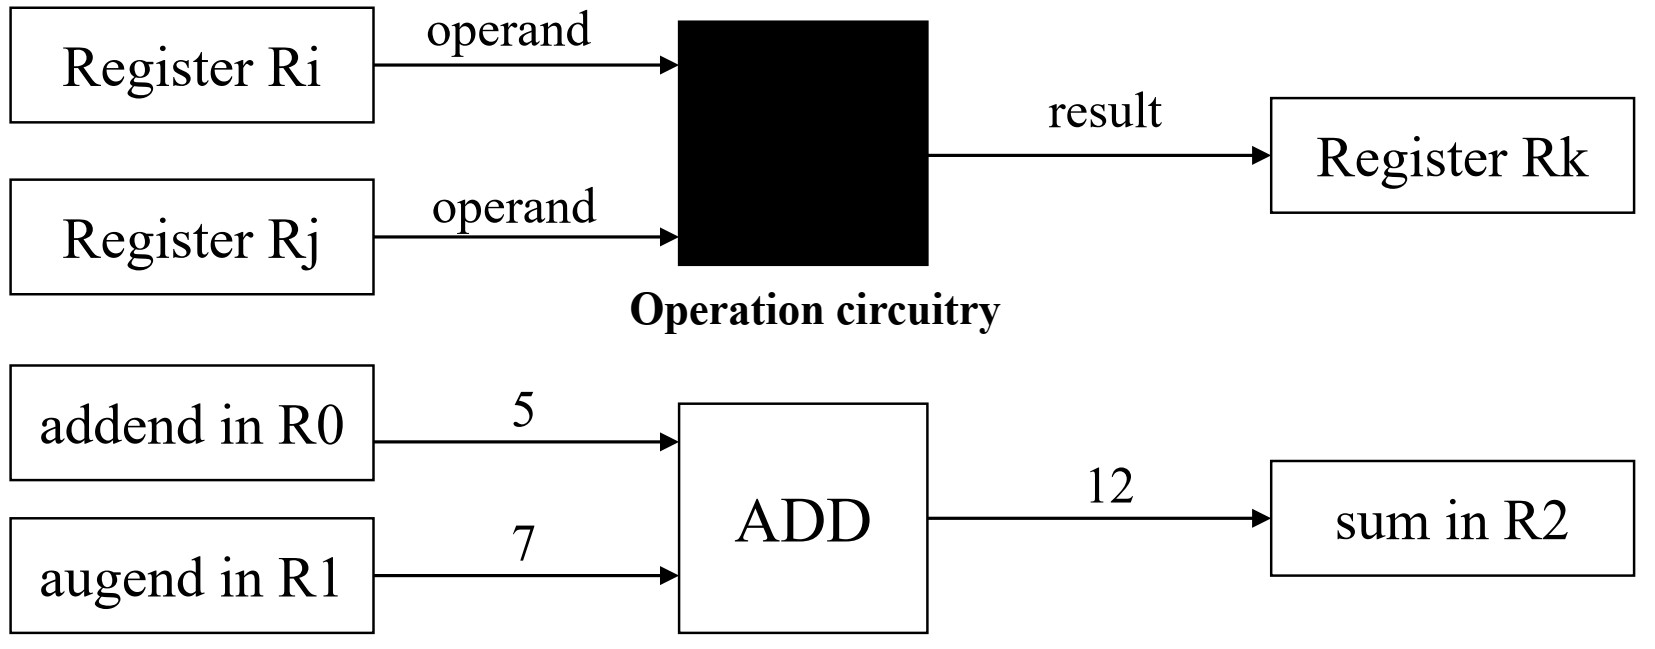
\includegraphics[scale=0.75]{registros.jpg}
		\end{frame}
		\begin{frame}{Que es un procesador multinúcleo?}
			\begin{itemize}
				\item Un CPU multicore es un chip con múltiples e independientes \textit{cerebros}, conocidos como núcleos
				\item Estos múltiples cores pueden correr programas completamente separados o pueden cooperar juntos para trabajar en paralelo en partes diferentes del mismo programa simultáneamente.
				\item Todos estos núcleos comparten la misma conexión a la memoria y la misma velocidad de conexión a esta (\textit{bandwidth})
			\end{itemize}
			El primer procesador (para la arquitectura x86) de un único núcleo fue lanzado por Intel en noviembre de 1971. En Junio y Julio de 2017, Intel lanzó un procesador de 28 núcleos y AMD uno de 32 núcleos, respectivamente.
		\end{frame}
	\subsection{Almacenamiento}
		\begin{frame}{Almacenamiento}
			Hay dos categorías principales de almacenamiento:
			\begin{itemize}
				\item Primaria
				\begin{itemize}
					\item Cache
					\item Memoria principal (RAM)
				\end{itemize}
				\item Secundaria
				\begin{itemize}
					\item Disco duro
					\item Desmontables (CD,USB,etc.)
				\end{itemize}
			\end{itemize}
		\end{frame}
		\begin{frame}{Almacenamiento primario}
			El almacenamiento primario es donde la información y las instrucciones están cuando ellos están por ser utilizados por un programa que esta corriendo en ese instante.
			\begin{itemize}
				\item Es volatil (regularmente): La información desaparecerá cuando la energía sea apagada.
				\item Típicamente tiene dos sub categorías:
				\begin{itemize}
					\item Cache
					\item Memoria principal (RAM)
				\end{itemize}
			\end{itemize}
		\end{frame}
		\begin{frame}{Cache}
			La memoria Cache es donde la información e instrucciones están cuando ellos van a ser usados muy muy pronto o han sido usados.
			\begin{itemize}
				\item El cache es muy rápido (entre el 5\% y el 100\% de la velocidad de los registros) comparado con la RAM ($\sim$ 1\% de la velocidad de los registros)
				\item Por tanto, es muy cara (Alrededor de \$ 20 USD por Mb)
				\item Por tanto, es muy pequeña (de 1 a 128 Mb)
			\end{itemize}
			A pesar de esto, es mucho más grande que los registros.
			
			Típicamente, la información se mueve entre el cache y el CPU a una velocidad cercana de la que el CPU realiza las operaciones.
		\end{frame}
		\begin{frame}{Memoria principal (RAM)}
			La memoria principal (RAM) es donde la información e instrucciones están y serán usadas en algún momento por un programa que está corriendo. Esta información puede ser usada pronto o no puede ser usada al final.
			\begin{itemize}
				\item Mucho más lento que el cache (Menos de 1\% de la velocidad de CPU) vs del 5-100\% de la velocidad del CPU para el cache)
				\item Por lo tanto, mucho mas barata que el cache. (\$ 0.0076 USD por MB para la ram)
				\item Por lo tanto, mucho mas grande que el cache (de 1GB a 1+ TB para la ram vs menos de 1 MB a 128 Mb para el cache)
			\end{itemize}			 
		\end{frame}
		\begin{frame}{Esquema de la memoria principal}
			\begin{columns}
				\begin{column}{0.4\textwidth}
					La memoria principal está echa de \textit{locations} también llamadas \textit{cells}.
					
					Cada \textit{location} tiene una dirección entera única que nunca cambia.
					
					Cada \textit{location} tiene un valor, también conocido como el \textit{contents}, que el CPU puede mirar y cambiar.
					
					Se pensará que la memoria es una línea continua de \textit{cells}
				\end{column}
				\begin{column}{0.6\textwidth}
					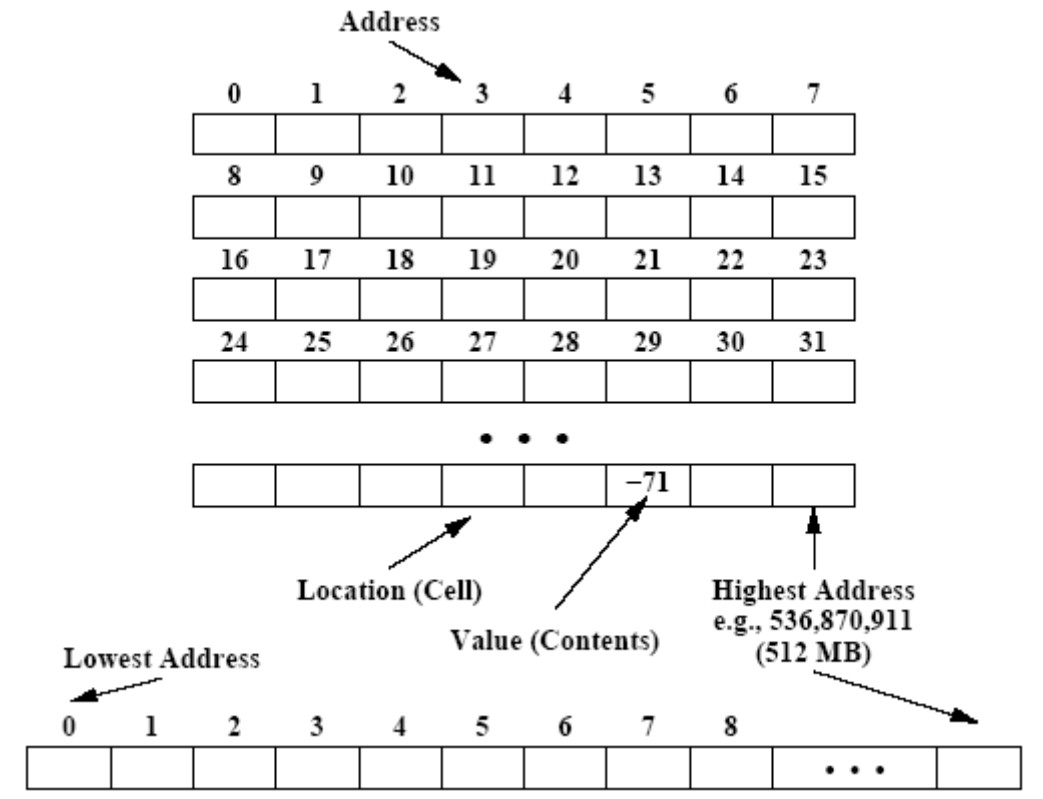
\includegraphics[width=\textwidth]{ram.jpg}
				\end{column}				
			\end{columns}
		\end{frame}
		\begin{frame}{RAM vs ROM}
			RAM: Random Access Memory
			\begin{itemize}
				\item Memoria que el CPU puede ver y cambiar arbitrariamente.
				\item La memoria principal, memoria y RAM son sinónimos (a menos de que se especifique lo contrario)
				\item Algunas veces se conoce como la memoria núcleo, este nombre es debido a la vieja tecnología de memoria
			\end{itemize}
			ROM: Read Only Memory
			\begin{itemize}
				\item Memoria que el CPU puede ver arbitrariamente pero no puede cambiar.
			\end{itemize}
		\end{frame}
		\begin{frame}{Velocidad =$>$ Precio =$>$ Tamaño}
			\begin{itemize}
				\item Los registros son muy rápidos, por que ellos están puestos directamente en el CPU
				\item También el cache es muy rápido, por que está puesto en el CPU, pero no está conectado directamente a la Unidad de Control o a la unidad Aritmética/lógica. Cache puede operar a velocidades similares a los registros, pero cache es mucho más grande que los registros (típicamente de de 1000 a 10000 veces más grande).
				\item La memoria principal es mucho más lenta que el cache ya que no es parte del CPU, por esto es mucho más barata que el cache y también por esto es mucho más grande que el cache (alrededor de 1000 veces más grande.)
			\end{itemize}
		\end{frame}
		\begin{frame}{Como viaja la información entre la RAM y el CPU}
			\begin{columns}	
				\begin{column}{0.5\textwidth}
					El bus es la conexión entre el CPU y la memoria principal por donde la información viaja.
					
					La velocidad de transferencia entre la RAM y el CPU es mucho más lenta que la velocidad de calculo del CPU, por lo que el CPU gasta mucho de su tiempo esperando a que la información llegue o salga.
					
					El CPU (i3 a 1.6Ghz) puede procesar hasta 653 GB/seg mientras que bus puede ser de 15 GB/seg	
				\end{column}
				\begin{column}{0.5\textwidth}	
					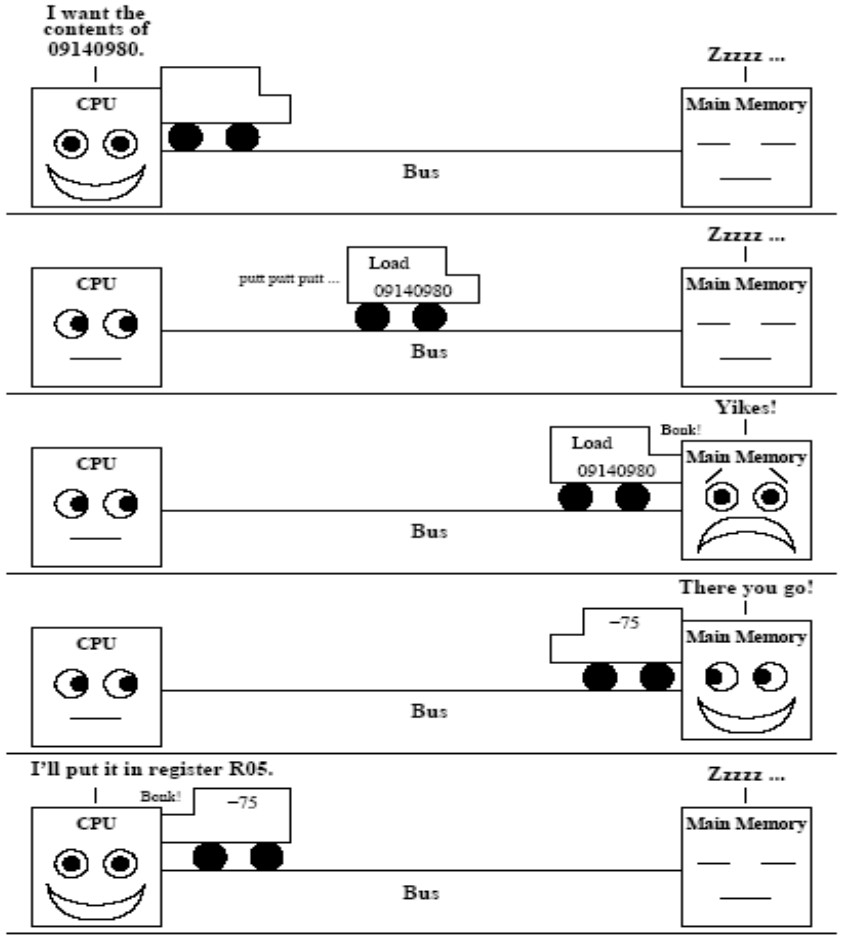
\includegraphics[width=\textwidth]{bus.jpg}
				\end{column}
			\end{columns}
		\end{frame}
		\begin{frame}{Por qué existe el cache?}
			El cache es mucho más rápido que la RAM, por lo que el CPU no tiene que esperar tanto ya que las cosas que necesita ya estarán en cache, por lo que puede hacer más operaciones por segundo.
			
			Por ejemplo, si se tiene un CPU (i3 a 1.7 Ghz) que pueda realizar 653 GB/seg y un cache que pueda procesar 46 GB/seg es un incremento a un bus que pueda procesar 15 GB/seg
		\end{frame}
		\begin{frame}{Almacenamiento secundario}
			\begin{itemize}
				\item La información y las instrucciones están aquí cuando generalmente van a ser usadas en un futuro
				\item No es volátil, es decir, no desaparecerá cuando sea apagada la computadora
				\item Es mucha más lenta que la ram, pero es mucho más rápida y grande.
				\item Generalmente pueden ser portátiles, es decir, que pueden ser desconectados y puestos en otra computadora de manera sencilla.
			\end{itemize}
		\end{frame}
		\begin{frame}{Tipos de dispositivos}
			\begin{itemize}
				\item Estado sólido
				\begin{itemize}
					\item Siempre se puede leer
					\item Siempre se puede escribir y reescribir en él varias veces
					\item No se borran con imanes
				\end{itemize}
				\item Magnético
				\begin{itemize}
					\item Siempre se puede leer
					\item Siempre se puede escribir y reescribir en él varias veces
					\item Se borran con imanes
				\end{itemize}
				\item Óptico
				\begin{itemize}
					\item Siempre se pueden leer
					\item En algunos solo se puede escribir una vez, en otros se puede reescribir varias veces
					\item No se borran con imanes
				\end{itemize}
				\item Papel: en desuso
			\end{itemize}
		\end{frame}
		\begin{frame}{Velocidad, precio y tamaño}
			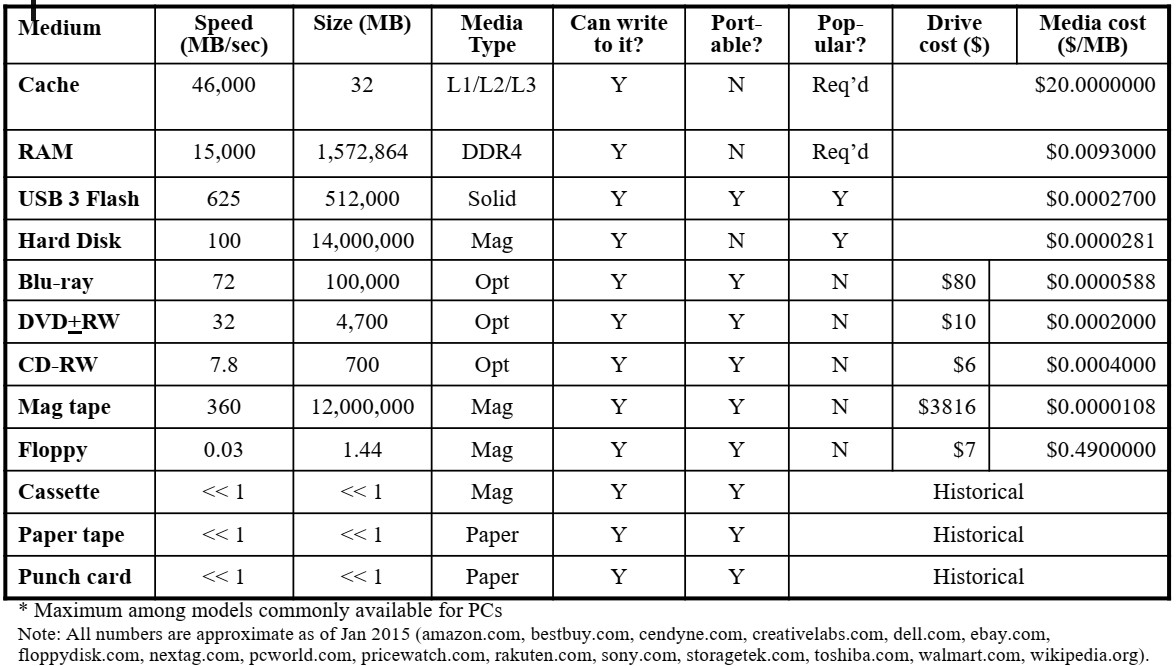
\includegraphics[width=\textwidth]{precio.jpg}
		\end{frame}
		\begin{frame}{CD-ROM/DVD-ROM/BD-ROM}
			Cuando un CD/DVD/Blu-ray guarda información, lo hace como \textit{Read Only Memory} (ROM)
			\begin{itemize}
				\item La información solo puede ser leída, no reescrita.
				\item No es volátil
				\item Puede tener dirección arbitraria (No es arbitraria, pero es tan rápida como si lo fuera)
			\end{itemize}
		\end{frame}
		\begin{frame}{CD-ROM/DVD-ROM/BD-ROM: Desventajas}
			Si lo comparamos con la memoria ROM, los disco son mucho más lentos que la memoria rom:
			\begin{itemize}
				\item CD-ROM a 7.8 MB/seg, DVD-ROM a 32 MB/seg, BD-ROM a 72 MB/seg. La memoria ROM puede ser 1000 veces mas rápida que un DVD o blu-ray y 2000 veces más que un CD
			\end{itemize}
		\end{frame}
		\begin{frame}{CD-ROM/DVD-ROM/BD-ROM: Ventajas}
			\begin{itemize}
				\item Precio: CD-ROM y DVD-ROM es mucho más barato que la ROM.
				\begin{itemize}
					\item BD-RE \$ 0.00006 por MB
					\item DVD-RW \$ 0.00020 por MB
					\item CD-RW \$ 0.00040 por MB
					\item es más cara que la RAM (\$ 0.0076 MB)
				\end{itemize}
				\item Tamaño: los CD y DVD son mucho más grande que la ROM, ya que esta está limitada a solo algunos GB.
			\end{itemize}
		\end{frame}
	\subsection{Entrada/Salida}
		\begin{frame}{I/O}
			I/O es una abreviación para \textit{Input/Output}.
			
			Los dispositivos de entrada transfieren información a la computadora. Por ejemplo:
			\begin{itemize}
				\item Teclado
				\item Ratón
				\item Scanner
				\item Micrófono
				\item Touchpad
				\item Joystick
			\end{itemize}
		\end{frame}
		\begin{frame}{I/O}
			Los dispositivo de salida transfieren información a afuera de la computadora.
			
			Por ejemplo:
			\begin{itemize}
				\item Monitor
				\item Impresora
				\item Bocinas
			\end{itemize}
			Hay dispositivos que pueden ser ambos tipos a la vez, por ejemplo, una touchscreen.
		\end{frame}
\section{Extra}
	\subsection{MotherBoard}
		\begin{frame}{Que es la MotherBoard?}
			La tarjeta madre permite a todas las partes de la computadora recibir energía y comunicarse con todas las demás.
			
			Las tarjetas madres han sido desarrolladas en los últimos 20 años. Las primeras tarjetas madre solo tenían algunos componentes de los que tienen actualmente.
			
			En los inicios, solo tenían el procesador y algunos puertos de tarjetas. Los usuarios conectaban los periféricos y las memorias en estos puertos.
			
			Actualmente, las tarjetas madres tienen una gran variedad de características que afectan directamente a las capacidades de la computadora.
		\end{frame}
		\begin{frame}{Mother Board}
			\begin{columns}
				\begin{column}{0.5\textwidth}
					Una MB es inservible por ella sola, pero cada computadora debe tener una para trabajar.
					
					Aunque cada tarjeta madre puede tener distintos componentes, debe tener al menos:
					\begin{itemize}
						\item Socket para el microprocesador
						\item Chipset que conecta el CPU con las otras partes de la computadora
						\item \textit{Basic Input\textbackslash Output System} (BIOS)
						\item Chip de reloj
					\end{itemize}										
				\end{column}
				\begin{column}{0.5\textwidth}
					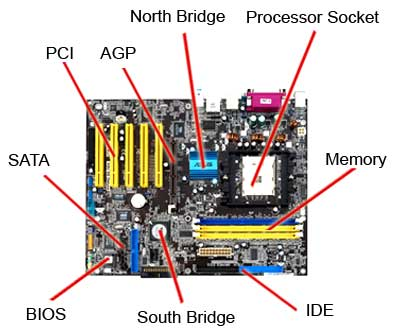
\includegraphics[scale=0.4]{mb.jpg}
				\end{column}
			\end{columns}
		\end{frame}
		\begin{frame}{MotherBoard}
			La tarjeta madre también puede incluir los siguientes puertos:
			\begin{itemize}
				\item Peripheral Component Interconnect (PCI)
				\item Accelerated Graphics Port (AGP)
				\item Integrated Drive Electronics (IDE)
				\item Puertos de memoria
			\end{itemize}
			Además de estos puertos, hay otros más nuevos como lo son PCI express o incluso los puertos SATA.
		\end{frame}
\end{document}